%%%%%%%%%%%%%%%%%%%%%%%%%%%%%%%%%%%%%%%%%
% Jacobs Landscape Poster
% LaTeX Template
% Version 1.1 (14/06/14)
%
% Created by:
% Computational Physics and Biophysics Group, Jacobs University
% https://teamwork.jacobs-university.de:8443/confluence/display/CoPandBiG/LaTeX+Poster
% 
% Further modified by:
% Nathaniel Johnston (nathaniel@njohnston.ca)
%
% This template has been downloaded from:
% http://www.LaTeXTemplates.com
%
% License:
% CC BY-NC-SA 3.0 (http://creativecommons.org/licenses/by-nc-sa/3.0/)
%
%%%%%%%%%%%%%%%%%%%%%%%%%%%%%%%%%%%%%%%%%

%----------------------------------------------------------------------------------------
%	PACKAGES AND OTHER DOCUMENT CONFIGURATIONS
%----------------------------------------------------------------------------------------

\documentclass[final]{beamer}

\usepackage[size=a0,orientation=portrait,scale=1.24]{beamerposter} % Use the beamerposter package for laying out the poster

\usetheme{confposter} % Use the confposter theme supplied with this template

\setbeamercolor{block title}{fg=ngreen,bg=white} % Colors of the block titles
\setbeamercolor{block body}{fg=black,bg=white} % Colors of the body of blocks
\setbeamercolor{block alerted title}{fg=white,bg=dblue!70} % Colors of the highlighted block titles
\setbeamercolor{block alerted body}{fg=black,bg=dblue!10} % Colors of the body of highlighted blocks
% Many more colors are available for use in beamerthemeconfposter.sty

%-----------------------------------------------------------
% Define the column widths and overall poster size
% To set effective sepwid, onecolwid and twocolwid values, first choose how many columns you want and how much separation you want between columns
% In this template, the separation width chosen is 0.024 of the paper width and a 4-column layout
% onecolwid should therefore be (1-(# of columns+1)*sepwid)/# of columns e.g. (1-(4+1)*0.024)/4 = 0.22
% Set twocolwid to be (2*onecolwid)+sepwid = 0.464
% Set threecolwid to be (3*onecolwid)+2*sepwid = 0.708

\newlength{\sepwid}
\newlength{\onecolwid}
\newlength{\twocolwid}
\newlength{\threecolwid}
\setlength{\paperwidth}{33.1in} % A0 width: 46.8in
\setlength{\paperheight}{46.8in} % A0 height: 33.1in
\setlength{\sepwid}{0.066\paperwidth} % Separation width (white space) between columns
\setlength{\onecolwid}{0.4\paperwidth} % Width of one column
\setlength{\twocolwid}{0.4\paperwidth} % Width of two columns
\setlength{\threecolwid}{0.8\paperwidth} % Width of three columns
\setlength{\topmargin}{-0.5in} % Reduce the top margin size
%-----------------------------------------------------------

\usepackage{graphicx}  % Required for including images

\usepackage{booktabs} % Top and bottom rules for tables

\usepackage{units}
\usepackage{subfig}

%----------------------------------------------------------------------------------------
%	TITLE SECTION 
%----------------------------------------------------------------------------------------

\title{Time Stretching of GeV Emission from GRBs:\\[0.2ex]Fermi LAT vs Geometrical Model} % Poster title

\author{Maxim Piskunov and Grigory Rubtsov \\[.3ex] \normalsize \href{mailto:maxit@ms2.inr.ac.ru}{maxit@ms2.inr.ac.ru}} % Author(s)

\institute{Institute for Nuclear Research RAS \\[2.0ex] \normalsize \url{https://github.com/maxitg/GammaRays}} % Institution(s)

%----------------------------------------------------------------------------------------

\begin{document}

\addtobeamertemplate{block end}{}{\vspace*{2ex}} % White space under blocks
\addtobeamertemplate{block alerted end}{}{\vspace*{2ex}} % White space under highlighted (alert) blocks

\setlength{\belowcaptionskip}{2ex} % White space under figures
\setlength\belowdisplayshortskip{2ex} % White space under equations

\begin{frame}[t] % The whole poster is enclosed in one beamer frame

\begin{columns}[t] % The whole poster consists of three major columns, the second of which is split into two columns twice - the [t] option aligns each column's content to the top

\begin{column}{\sepwid}\end{column} % Empty spacer column

\begin{column}{\onecolwid} % The first column



%----------------------------------------------------------------------------------------
%	INTRODUCTION
%----------------------------------------------------------------------------------------

\begin{block}{Introduction}

Observations confirm that the high energy $(> \unit[100]{MeV})$ emission of gamma ray bursts is delayed with respect to the low energy emission.
However, the difference of light curves in various high energy bands has not been studied properly.
We study GRBs in two energy bands: \unit[100]{MeV} to \unit[1]{GeV}, and \unit[1]{GeV} to \unit[300]{GeV}.

\end{block}

%------------------------------------------------

\begin{block}{Observations}

\begin{figure}
{\large Kolmogorov-Smirnov test results for GRB 090926A} \\[0.5ex]
\subfloat{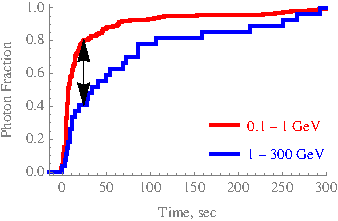
\includegraphics[width=\textwidth]{lightCurveArrow090926A}} \\
\subfloat{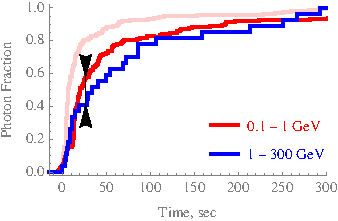
\includegraphics[width=\textwidth]{lightCurveStretchedArrow090926A.pdf}} \\
\end{figure}

\begin{itemize}
\item{4 GRBs were studied: 080916C, 090510, 090902B and 090926A.}
\item{080916C and 090902B have stretching factors compatible with 1 within $2\sigma$.}
\item{High energy light curve of 090926A is stretched with respect to low energy one (with $3.3\sigma$ significance)}
\item{Low energy light curve of 090902B is stretched with respect to high energy one (with $2.2\sigma$ significance)}
\end{itemize}

\end{block}

%----------------------------------------------------------------------------------------

\end{column} % End of the first column

\begin{column}{\sepwid}\end{column} % Empty spacer column

\begin{column}{\twocolwid} % Begin a column which is two columns wide (column 2)

\begin{columns}[t,totalwidth=\twocolwid] % Split up the two columns wide column

\begin{column}{\onecolwid}\vspace{-.6in} % The first column within column 2 (column 2.1)

%----------------------------------------------------------------------------------------
%	MATERIALS
%----------------------------------------------------------------------------------------

\begin{block}{Model}

\begin{figure}
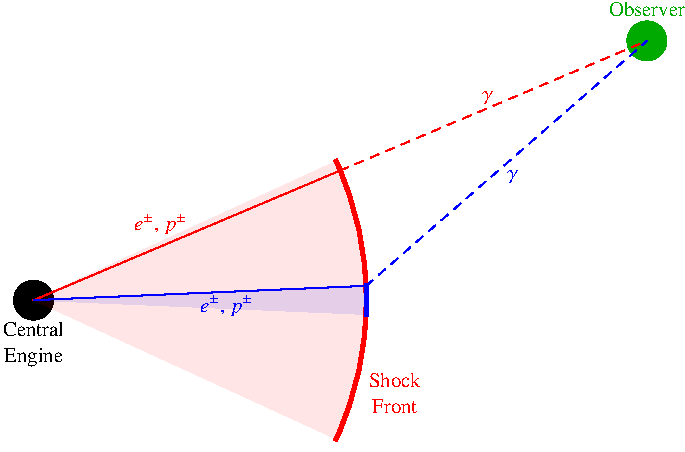
\includegraphics[width=\textwidth]{modelOverview.pdf}
\end{figure}

We suggest a simple geometrical model to explain this result.
The main hypothesis is the jet opening angle dependence on radiation energy -- the most energetic photons are emitted near the axis of the jet.

\begin{enumerate}
	\item{Time $t = 0$, the central engine emits a spherical shell of plasma.}
	\item{The shell propagates with relativistic velocity.}
	\item{Each jet point is an isotropic radiator in its inertial reference frame.}
	\item{
		Intensity depends on coordinates in space and frequencies:
		\begin{equation*}
			\eta\left(r,\theta,\omega\right) = 
			\frac{\eta_0}{1 + \left(r/r_0\right)^n}
			e^{
				-\left(\theta/\theta_0\right)^2
				\left(\omega/\omega_0\right)^{-2k}
			}
			\left(\omega/\omega_0\right)^\alpha
		\end{equation*}
	}
\end{enumerate}

\end{block}

\begin{block}{Results}

The simple geometrical model can explain observed stretching:

\begin{figure}
	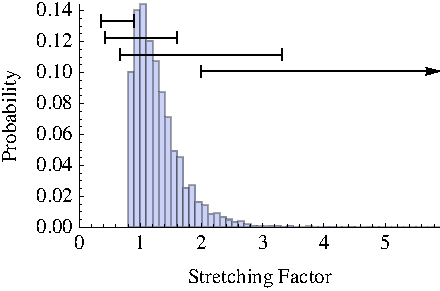
\includegraphics[width=\textwidth]{kappaDistributionHistogram}
\end{figure}

We also computed (for some parameter values):

\begin{itemize}
	\item{Total energy of the burst above \unit[1]{GeV}. The result is reasonable.}
	\item{Fraction of bursts observable above \unit[100]{MeV}, which are also observed above \unit[1]{GeV} is $f_m = 0.072$. Observed value is $f_o = 0.086$.}
\end{itemize}

\end{block}

%----------------------------------------------------------------------------------------

\end{column} % End of column 2.1

\end{columns} % End of the split of column 2 - any content after this will now take up 2 columns width

%----------------------------------------------------------------------------------------



\end{column} % End of the second column

\begin{column}{\sepwid}\end{column} % Empty spacer column


\end{columns} % End of all the columns in the poster

\end{frame} % End of the enclosing frame

\end{document}
